% add to Table of content
\addcontentsline{toc}{section}{\bf{APPENDIX B: TITLE}}

% set 0 indentation
\setlength{\parindent}{0pt}
% set paragraph space = 1 space
\setlength{\parskip}{1em}
% set line space = 1.5
\setlength{\baselineskip}{1.5em}

\renewcommand{\thefigure}{B\arabic{figure}}
\renewcommand{\thetable}{B\arabic{table}}

\begin{center}
  \fontsize{14}{17}\selectfont{\textbf{
    APPENDIX B
  }}\\
  \fontsize{14}{25}\selectfont{\textbf{
    TITLE
  }}
\end{center}
% \vspace{1em}

Multiple texts, tables and/or figures can be combined in one appendix.  They should be referred to in a section or parts of your thesis. Number and title the materials in the order they are mentioned in the sections. Add a short description of Appendix A.  Do the same for other appendices with multiple materials.

\begin{figure}[ht]
  \centering
  \caption[CCTV monitoring room in Appendix B.]{CCTV monitoring room. Reprinted from the Twenty First Security Web site (\url{http://www.twentyfirstsecurity.com.au/}).}
  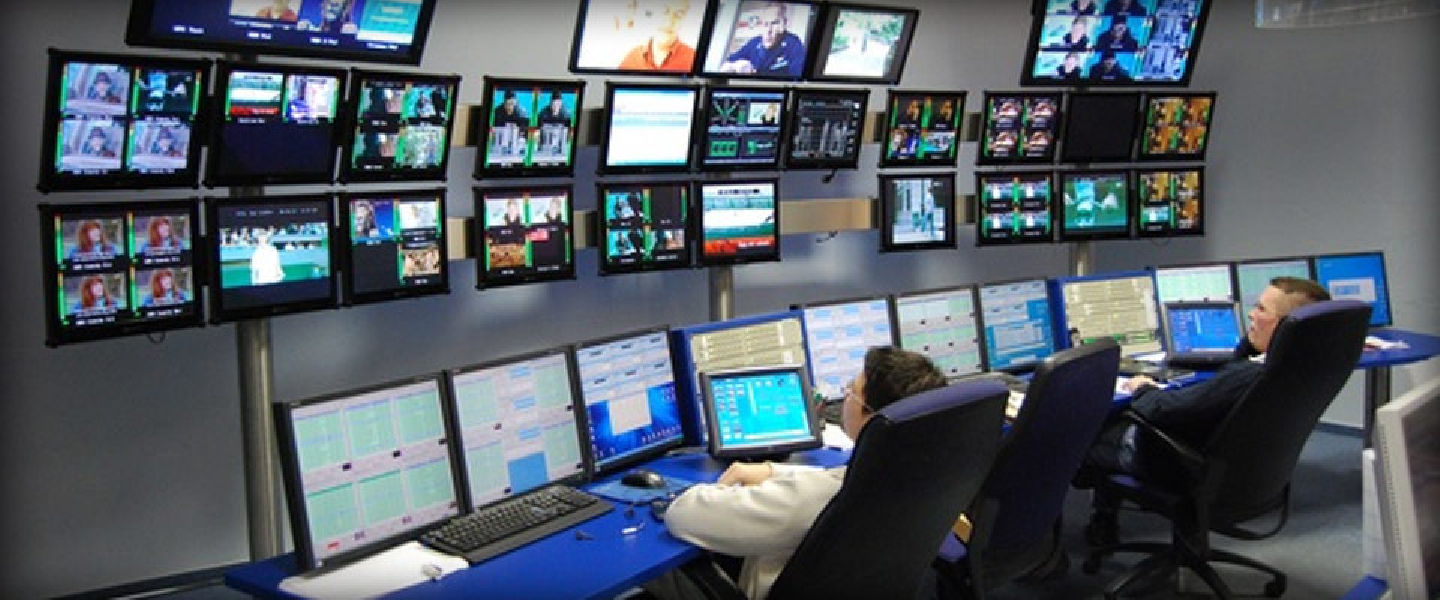
\includegraphics[width=5in]{figures/monitoring}
  \label{fig:monitoring-test}
\end{figure}

\begin{table}[ht]
  \caption[Random Table B]{Random Table B}
  \begin{center}
    \begin{tabular}{cccc}
      \hline \textbf{v1} & \textbf{v2} & \textbf{v3} & \textbf{Overall} \\ \hline
        78.67\% & 87.33\% & 94.92\% & 85.64\% \\ \hline
    \end{tabular}
  \end{center}
  \label{tab:random_table_B}
\end{table} 